||\documentclass[11pt]{article} % do not change this line
\input{BigDataStyle.txt}      % do not change this line
\usepackage{amsmath,amsfonts,amssymb,amsthm,latexsym,graphicx,caption}
\usepackage[boxed,ruled,vlined,linesnumbered,dotocloa,english,onelanguage]{algorithm2e}
\graphicspath{ {pictures/} }
\emergencystretch=5mm
\tolerance=400
\allowdisplaybreaks[4]

\theoremstyle{plain}
\newtheorem{theorem}{Theorem}[section]
\newtheorem{proposition}[theorem]{Proposition}
\newtheorem{corollary}[theorem]{Corollary}
\newtheorem{lemma}[theorem]{Lemma}
\newtheorem{problem}[theorem]{Problem}
\newtheorem{definition}{Definition}[section]

\theoremstyle{definition}
\newtheorem*{remark}{Remark}

\title{Analysis of Symmetry Breaking Algorithms}
\author{Marcos Tileria}

\newcommand{\Programme}{MSc Distributed and Networked Systems}
% Computational Finance students: uncomment the next line
%\twodepartmentstrue

\begin{document}
\maketitle

\declaration

\begin{abstract}
  
Breaking symmetry is a very well study problem in distributed computing. A distributed system is composed of nodes with an initial state, possibly the same for every node and a set of edges between the nodes. The aim of symmetry breaking is to break the initial state of symmetry between the nodes to perform some computation. Synchronous algorithm provides an easy mechanism to design and study protocols. The objective of this dissertation is to simulate a synchronous message passing system and analyse time and message complexity of the Maximal Independent Set problem, which is one of the most important breaking symmetry problem. To simulate the synchronous message passing system, three types of synchronization techniques are used and an analysis of the trade off between these techniques is presented. A simulator build in Elixir using the actor model was developed to test the MIS algorithm with different synchronizations techniques. TO BE COMPLETE AFTER TESTS 
  
\end{abstract}

\section{Introduction}

\section{Introduction}
\label{cap:1}

One of the central problem in distributed computing is called Symmetry Breaking. This problem occurs when all processors in a network are in the same state, possibly with a unique identifier. This state of symmetry should be broken before beginning any computation. Some examples of symmetry breaking problems are computing the maximal independent sets \textit{(MIS)} , maximal matching, vertex colouring, ruling sets and leader election. This project focus on the problem of finding the maximal independent set on an undirected graph using the local model \cite{linial1992locality}.

In the local model, each vertex of the graph is occupied by a processor and has a unique identifier ID. The processors only communicate with each other by sending messages, there is no notion of shared memory. Locality in distributed networks means that in order to obtain the solution of a general problem, a processor only uses locally available data. In this model, computation is assumed to be reliable and synchronous. No faulty processors are permitted in this model and every processor executes the local algorithm in steps call rounds. 

An independent set \textit{IS} of an undirected graph is a subset S of nodes such that no two nodes in S are adjacent. An \textit{IS} is considered maximal if no extra node can be added to \textit{IS} without violating the independence. The \textit{MIS} problem is one of the most important problem in the area of local graph algorithm because many other problems like graph colouring can be reduced to it \cite{panconesi1992improved}. A maximum independent set \textit{MaxIS} is a \textit{MIS} of maximum cardinality, this problem, in contrast to \textit{MIS} in NP-hard. In this project a random-priority parallel algorithm developed by Yves \textit{et al.} \cite{yves2009optimal} is used in order to find the MIS of a given graph.


There are many applications of the \textit{MIS}, for instance: resource scheduling, topology control in wireless sensor networks \cite{basagni2001finding}, analysis of biological systems \cite{afek2013beeping}. Karp and Wigderson \cite{karp1986constructing} presented reductions from others graph theory problems (Maximal Set Packing, Maximal Matching, 2-Satisfiability) to the \textit{MIS} and proved that the \textit{MIS} problem is in NC.


In practice, the majority of the distributed systems are asynchronous, however, protocols are easy to design and implement in the synchronous model. Once that an algorithm has been designed in the synchronous model it can be transformed to an asynchronous algorithm.  The main reason why synchronous algorithms are easy to design is that the model makes strong assumptions and put constraints that restrict the behaviour of the system.


There are many techniques to simulate a synchronous system over an asynchronous system. A synchronizer is a simulation from the synchronous system to the asynchronous system. These simulations can be local or global. In a local simulation, processors only keep the synchronization with its neighbours, on the contrary, on global simulations all processors are synchronized.  For this reason, with local synchronization, especially in large networks, processors might be in different rounds. For this project, two well know synchronizers proposed by Awerbuch \cite{awerbuch1985complexity} are used, Alpha and Beta Synchronizer. Besides, a global synchronizer with a master processor that controls the synchronization was implemented to analyse the overhead generated by different techniques in terms of messages and time.




The rest of the report is organised as follow: The next section presents relevant work about symmetry breaking, maximal independent set and synchronizers. Section \ref{cap:2} presents the background of symmetry breaking and define the MIS problem. Different approaches to simulate synchronous systems are discussed in Section \ref{chap:3}. A description of the simulator and a tutorial on how to use it is given in section \ref{chap:4} The experimental settings of the simulations are explained in Section \ref{chap:5}. Section \ref{chap:6} gives the evaluation of results and conclusion. Finally, the professional issues are presented in Section \ref{chap:7}. 

\subsection{Background Research}
 
Deterministic and randomised algorithms are two well studied approaches to solve symmetry breaking problem. Usually, randomisation provide simpler and faster implementation than the deterministic counterpart. Deterministic algorithm always reaches the solution of the problem, in contrast, randomised algorithms achieve termination with high probability. Relevant work, especially the ones related to \textit{MIS} problem are quoted below.

In \cite{luby1986simple}, Luby proposes the first solution to the \textit{MIS} problem using a simple randomised algorithm. The same year Alon \textit{et al.} present in \cite{alon1986fast} another randomised solution and made a comparison with others algorithms that were turned from randomised to deterministic. Both algorithms run in $O(\log |N|)$ in general graphs. In \cite{linial1992locality} Linial present a $\Omega(\log* |N|)$ algorithm to find the MIS for n-cycle graphs. A deterministic solutions was presented by Panaconesi \textit{et al.} in \cite{panconesi1996complexity} that run in $2^{O\sqrt{\log N}}$, more recently, many deterministic algorithms were presented by Barenboim and Elkin in \cite{barenboim2010sublogarithmic} with different running times for different network topologies. Schneider and Wattenhofer developed a $O(\log^* N)$ deterministic algorithm for graphs with bounded growth in \cite{barenboim2010sublogarithmic}. In \cite{yves2009optimal}, Ives \textit{et al.} present a variant of the original Luby's algorithm with optimal bit complexity for the messages sent over the network, this algorithm is used in this project for testing purpose.

 

In \cite{awerbuch1985complexity}, Awerbuch present a general simulation technique to allow the implementation of algorithm in synchronous networks, referred to as synchronizer. In this paper, the author present three synchronizer Alpha, Beta and Gama, which are a generalisation of the work of Gallager and Robert in \cite{gallager1982distributed}. Logical buffering is another technique to simulate synchronization and was independently developed by Welch in \cite{welch1987simulating} and Neier and Toueg in \cite{neiger1993simulating}. Others techniques were developed improving the synchronizer mention before under some restrictions, for example, Peleg in \cite{peleg1989optimal} for multidimensional mesh network with two nodes in each dimension(hyper-cube).

 Barenboim \textit{et al.} made in \cite{barenboim2016locality} a survey of symmetry breaking algorithms describing the main results achieved on the topic and proposed new algorithms for the most popular symmetry breaking problems: \textit{MIS}, maximal matching, vertex colouring and ruling sets. In \cite{johnson1985symmetry} Johnson and Schneider present a discussion to address the meaning of symmetry and introduce the concept of similarity.  
\newline



\section{The Symmetry Breaking Problem}
\label{cap:2}

Formally, a symmetry system can be defined as a system in which the processes are in an equivalence relation, this means that if the processes run the same code, it is possible to permute the processes without changing the behaviour of the system. One example of this state would be a ring in which there is no unique identifier for every processes \cite{boldi1996symmetry}. 

If we consider a message passing system in which exist an initial state of symmetry between all processes, it is possible to find a synchronous execution in which the processes will continue in the same initial state. In this case, it is necessary a mechanism to break the symmetry, on the contrary, the system cannot escape from the initial state.
%as shown in \cite{angluin1980local} by Angluin.

Symmetry breaking is one of the most extensively studied problems in distributed computing. The fundamental problems on graph include the maximal matching, vertex colouring, ruling sets and \textit{MIS}. The last one can be considered as the central problem because all the others can be reduced to it, as shown in  \cite{linial1992locality}.

In the next section, a formal definition of the maximal independent set is given. A  discussion on the sequential algorithm vs distributed algorithm is presented with the theoretical analysis on time complexity and message complexity in the case of the distributed approach. Henceforth the terms vertices and processes are used in the same context and are interchangeable.    

\subsection{Maximal Independent Set}

\theoremstyle{definition}
\begin{definition}

Given a undirected graph $G = (V,E)$, a Maximal Independent Set \textbf{MIS} is a set of vertices $S \subseteq V$ if it satisfied the following properties:   

\begin{enumerate}
  \item the set S in an independent set meaning that no two vertices $v,u \in S$ are adjacent,
  \item the set S is maximal, with regards to independence, meaning that for each vertex $v \notin S$, there exist a neighbour $u$ of $v$ such that $u \in S$.
\end{enumerate}

\end{definition}

REWRITE THIS PARAGRAPH
Figure \ref{fig:graph1} show an example of undirected graph $G$ with 8 vertices and 14 edges. The goal is to find a MIS of $G$, informally, a set of vertices in which every vertex $v$ is part of the set or a neighbour of $v$ is part of the set. It is possible to find more that one solution to the same instance as shown in the example.
 
\begin{figure}[ht]
\centering
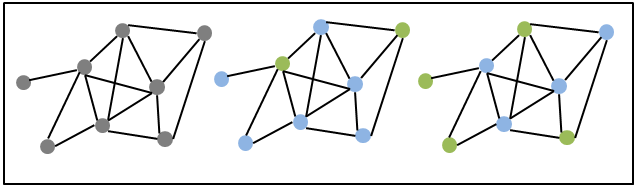
\includegraphics[width=1 \linewidth, height=5cm]{mis-example.PNG} 
\caption{Maximal Independent Set of a general graph}
\label{fig:graph1}
\end{figure}


The algorithm \ref{algorithm:secuential-mis} describe a general sequential algorithm to find the maximal independent set of a general graph. The time complexity is $O(N)$ since in the worst case, the algorithm has to check every vertex. Another approach to improve this time is desirable. In the next section, two distributed algorithm to find the \textit{MIS} are presented.

\begin{algorithm}
 \caption{Sequential Maximal Independent Set}
 \label{algorithm:secuential-mis} 

\SetAlgoNoLine
\KwResult{IS Set of vertices}
\KwData{ $G(V,E)$ Graph}
    \While {V is not empty}{
        Choose a vertex $v \in V$
            Add v to the set IS\;
            Remove from V the vertex v and all its neighbours\;
        }
    
 
\end{algorithm}
 
 


 
\subsection{Distributed Maximal Independent Set}

A logarithmic lower bound is always desirable to solve a problem optimally, for this reason, the difficulty to find it in sequential algorithms motivated the proposal of distributed algorithms. In distributed computing, randomised algorithm is a powerful and efficient technique to solve efficiently problem that may take longer time in deterministic approach.

In 1986, a efficient distributed algorithm was proposed independently by Luby \cite{luby1986simple} and Alon \textit{et al.} \cite{alon1986fast}. Both algorithms are randomised and have $O(log N)$ lower bound. Until now, there are faster than the best deterministic algorithms for general graphs. There have been some improvements for special cases, for instance, \cite{panconesi1996complexity} propose a $O(\delta + log^* N)$ algorithm for specific graphs, however, the original algorithms are still faster when the running time is expressed as a function of $N$. It is worth to mention that all algorithms exposed forward are in the synchronous model.  

The algorithm\ref{algorithm:luby-mis} describe the original Luby's algorithm. Show the correctness of this algorithm is very simple. In each round, if a vertex joins the set \textit{S}, no other neighbour join the set in the actual round or in any other round. The algorithm at the end produces a \textit{MIS} because the vertices with the highest degree will decide to enter the \textit{MIS} in each round until all vertices become inactive.

% If Luby’s algorithm ever
% terminates, then the final set S satisfies the
% independence property.

% Theorem 6: If Luby’s algorithm ever
% terminates, then the final set S satisfies the
% maximality property.

% \theoremstyle{definition}
\begin{definition}

An algorithm terminates w.h.p. (with high probability) within $O(t)$ time if it does so with probability at least $1 − 1/n^c$ for any choice of $c ≥ 1$.

\end{definition}

 Message complexity depends on the number of processes which are active in each phase and its denoted by $O(m)$ in \cite{luby1986simple}. With high probability $(1-1/n)$, the Luby's algorithm finishes  $4\log N$ round. The time complexity demonstration is omitted FOR THE MOMENT.

% \theoremstyle{theorem}
\begin{theorem}

Algorithm \ref{algorithm:luby-mis} computes a maximal independent set for any graph  in $O(\log n)$  rounds with high probability.

\end{theorem}


\begin{algorithm}
 \caption{Luby's Algorithm, code for each process $p_i$ i = 1 to N}
 \label{algorithm:luby-mis} 

\SetAlgoNoLine
\KwResult{MIS Maximal Independent Set}
\KwData{ $G(V,E)$ Graph}
    \While {V is not empty}{
        Choose a random set of vertices $S ⊆ V$, by selecting each vertex $v$ independently with probability $1/(2d(v))$, where d is the degree of $v$\;
        For every edge in E, if both its endpoints are in the random set S, then remove from S the endpoint whose degree is lower. Break ties arbitrarily, e.g. using a lexicographic order on the vertex names\;
        Add the set S to IS\;
        Remove from V the set S and all the neighbours of vertices in S\;
        }
\end{algorithm} 



The algorithm \ref{algorithm:main-mis} is another randomized distributed algorithm and was proposed by Yves \cite{yves2009optimal}. This algorithm is used for the simulations in this project. The rounds can be split into 2 phases for simplicity. In each phase, each process chooses a random value, send to its neighbours and wait to receive the value from all its neighbours. If the process has the maximum value, the join the set and output in. In the second phase, if the process decided to join the $MIS$, then send messages to all its actives neighbours. If the process receives a message from one neighbour, decide not join the MIS and output out. At the end of this phase, every process that made a decision about join or not the \textit{MIS} become inactive for the next rounds.

\begin{algorithm}
 \caption{MIS Algorithm, code for each process $p_i$ from i = 1 to N}
 \label{algorithm:main-mis} 

\SetAlgoNoLine
\KwResult{MIS Maximal Independent Set}
\KwData{ $G(V,E)$ Graph}
    \While {V is not empty}{
        Selects a random number $r(v)$ between [0,1] and sends to its neighbours\;
        If $r(v) < r(w)$ for all neighbours $w \in N(v)$ numbers, remove myself from V and enter to the MIS \newline
        Inform my neighbours that I am a MIS member and terminate\;
        If I heard that my neighbour is MIS, remove myself from the V and terminate\;
        }
\end{algorithm}

% Lemma 7.14 (Edge Removal). In a single phase, we remove at least half of
% the edges in expectation.

The correctness is very intuitive and similar to the Luby's algorithm. In one phase, one process $p_i$ join the set $S$ only if it has the larger value between its neighbours, at the end of that phase, all the $p_i$ neighbours become inactive. In consequence, there is no neighbour process in the $S$. This set $S$ is maximal because at least one vertex (with the global smallest value) will enter the $S$ per round, hence there is a progress in each round. If at some round, a vertex has no neighbours, automatically join $S$ and become inactive. This sequence continues in following rounds until every process becomes inactive

% \theoremstyle{theorem}
\begin{theorem}

Algorithm \ref{algorithm:main-mis} computes a maximal independent set for any graph in $O(\log n)$ rounds with high probability.

\end{theorem}


% . This algorithm operates in synchronous rounds. In line 2, every process select a random number to in order to break the symmetry with its neighbours, line 3 makes sure that if a vertex v join the MIS, no other neighbour of v join the MIS at the same time, this is true because the execution  occurs in rounds. the line 4 makes sure that any vertex that has a neighbour in the MIS, join the MIS at any point. 


\newpage


\section{Synchronous Simulation}

\section{Experimental Results}

\section{Conclusion}

\section{Professional Issues}


\bibliographystyle{plain}
\bibliography{bibliography}
\end{document}
